%%%%%%%%%%%%%%%%%%%%%%%%%%%%%%%%%%%%%%%%%
% Stylish Article
% LaTeX Template
% Version 2.1 (1/10/15)
%
% This template has been downloaded from:
% http://www.LaTeXTemplates.com
%
% Original author:
% Mathias Legrand (legrand.mathias@gmail.com) 
% With extensive modifications by:
% Vel (vel@latextemplates.com)
%
% License:
% CC BY-NC-SA 3.0 (http://creativecommons.org/licenses/by-nc-sa/3.0/)
%
%%%%%%%%%%%%%%%%%%%%%%%%%%%%%%%%%%%%%%%%%

%----------------------------------------------------------------------------------------
%	PACKAGES AND OTHER DOCUMENT CONFIGURATIONS
%----------------------------------------------------------------------------------------

\documentclass[fleqn,10pt]{SelfArx} % Document font size and equations flushed left

\usepackage[english]{babel} % Specify a different language here - english by default

\usepackage{lipsum} % Required to insert dummy text. To be removed otherwise

\usepackage{tikz}

%----------------------------------------------------------------------------------------
%	COLUMNS
%----------------------------------------------------------------------------------------

\setlength{\columnsep}{0.55cm} % Distance between the two columns of text
\setlength{\fboxrule}{0.75pt} % Width of the border around the abstract

%----------------------------------------------------------------------------------------
%	COLORS
%----------------------------------------------------------------------------------------

\definecolor{color1}{RGB}{0,0,90} % Color of the article title and sections
\definecolor{color2}{RGB}{0,20,20} % Color of the boxes behind the abstract and headings

%----------------------------------------------------------------------------------------
%	HYPERLINKS
%----------------------------------------------------------------------------------------

\usepackage{hyperref} % Required for hyperlinks
\hypersetup{hidelinks,colorlinks,breaklinks=true,urlcolor=color2,citecolor=color1,linkcolor=color1,bookmarksopen=false,pdftitle={Title},pdfauthor={Author}}

%----------------------------------------------------------------------------------------
%	ARTICLE INFORMATION
%----------------------------------------------------------------------------------------

\JournalInfo{F20RO Intelligent Robotics} % Journal information
\Archive{Robotics Project} % Additional notes (e.g. copyright, DOI, review/research article)

\PaperTitle{Elevated Plus Maze} % Article title

\Authors{Clarissa Cremona\textsuperscript{1}, Helmi Fraser\textsuperscript{2}} % Authors


\affiliation{} % Corresponding author

\Keywords{} % Keywords - if you don't want any simply remove all the text between the curly brackets
\newcommand{\keywordname}{Keywords} % Defines the keywords heading name

%----------------------------------------------------------------------------------------
%	ABSTRACT
%----------------------------------------------------------------------------------------
\addto\captionsenglish{%
	\renewcommand{\abstractname}{}
}
 \Abstract{\textbf{Group 5}: \textsuperscript{1} cc531@hw.ac.uk, \textsuperscript{2} hmf30@hw.ac.uk}

%----------------------------------------------------------------------------------------

\begin{document}

\flushbottom % Makes all text pages the same height

\maketitle % Print the title and abstract box


%----------------------------------------------------------------------------------------
%	ARTICLE CONTENTS
%----------------------------------------------------------------------------------------

\pagenumbering{arabic}
\section{Introduction} % The \section*{} command stops section numbering

The elevated plus maze is a widely used experimental apparatus for measuring anxiety in rodents. Historically, it was first used in the 1950s in order to analyse the approach/avoidance conflict in rats exposed to a new environment. More recently, it has been used to test the effects of behaviour modification drugs by observing the movements of the rat before and after exposure.

In this report, a method of developing a computational model to simulate the behaviour of a rodent in this maze is described. This was achieved by using a genetic algorithm to evolve a feed-forward multi-layer perceptron controlling the movements of the robot.




\section{Background}
%------------------------------------------------

%\begin{enumerate}[noitemsep] % [noitemsep] removes whitespace between the items for a compact look
%\item First item in a list
%\item Second item in a list
%\item Third item in a list
%\end{enumerate}

\subsection{Elevated Plus Maze}

Initially conceived in 1955 by K. C. Montgomery, the elevated plus maze was a way to study the simultaneous feelings of curiosity and fear that rats experience when exposed to a new environment. \cite{Montgomery1955}

The elevated plus maze is a four-arm, raised platform in the shape of a plus sign. The maze consists of two enclosed arms and two open arms, perpendicular to the enclosed. \cite{Carter2010} It is one of the most widely used and validated tests for measuring the anxiety responses of rats under variety of conditions. \cite{Walf2007}

As a result of early experiments, it was found that the rodent tends to spend more time in the enclosed arms. The behaviour observed within these experiments is as a result of the approach/avoidance conflict when a rat is within a new environment. \cite{Lister1987} It was common to record the behaviour of the animal for 5 minutes, as it was found that after this time, rats would acclimatise to their environment and its behaviour would change. \cite{Komada2008}

\subsection{E-puck}

Developed by \citeauthor{epfl-epuck} at the Autonomous Systems Lab of \'{E}cole Polytechnique F\'{e}d\'{e}rale de Lausanne (EPFL), the E-puck (see Fig \ref{fig:epuck-pic}) is  an open source, two wheeled, differential robot measuring roughly 7cm in diameter. \cite{epfl-epuck}

\begin{figure}[H]
	\centering
	\begin{minipage}{.5\textwidth}
		\centering
		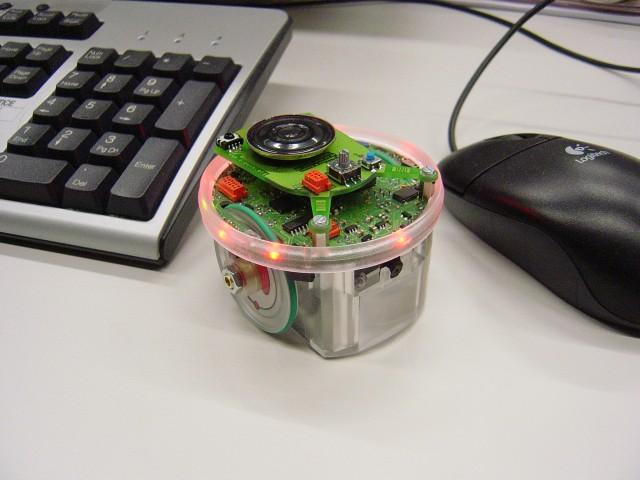
\includegraphics[width=.85\linewidth]{epuck}
		\captionof{figure}{E-puck mobile robot}
		\label{fig:epuck-pic}
	\end{minipage}%
\end{figure}

\begin{figure*}[!ht]
	\centering
	\def\layersep{2cm}
	\def\hiddenlayers{1}
	\def\hiddenneurons{2}
	
	\def\hiddenlayernodes{3}
	
	\begin{tikzpicture}[shorten >=1pt,->,draw=black!50, node distance=\layersep]
	\tikzstyle{every pin edge}=[<-,shorten <=1pt]
	\tikzstyle{neuron}=[circle,fill=black!25,minimum size=17pt,inner sep=0pt]
	\tikzstyle{input neuron}=[neuron, fill=cyan!50];
	\tikzstyle{output neuron}=[neuron, fill=black!50];
	\tikzstyle{hidden neuron}=[neuron, fill=purple!50];
	\tikzstyle{annot} = [text width=4em, text centered]
	
	% Draw the input layer nodes
	\foreach \name / \y in {0,...,7}
	% This is the same as writing \foreach \name / \y in {1/1,2/2,3/3,4/4}
	\node[input neuron, pin=left:IR Sensor \y] (I-\name) at (0,-\y) {};
	
	% Draw the hidden layer nodes
	\foreach \name / \y in {0,...,\hiddenlayernodes}
	\path[yshift=-2cm]
	node[hidden neuron] (H-\name) at (\layersep,-\y cm) {};
	
	
	% Draw the output layer node
	\node[yshift=0][output neuron,pin={[pin edge={->}]right:Left Speed}, right of=H-1] (O-1) {};
	\node[yshift=0][output neuron,pin={[pin edge={->}]right:Right speed}, right of=H-2] (O-2) {};
	
	% Connect every node in the input layer with every node in the
	% hidden layer.
	\foreach \source in {0,...,7}
	\foreach \dest in {0,...,\hiddenlayernodes}
	\path (I-\source) edge (H-\dest);
	
	
	% Connect every node in the second hidden layer with the output
	\foreach \source in {0,...,\hiddenlayernodes}
	\foreach \dest in {1,...,2}
	\path (H-\source) edge (O-\dest);
	
	% Annotate the layers
	\node[xshift=0cm][annot,above of=I-1] (first) {Input layer};
	\node[xshift=1cm][annot,right of=first, node distance=1cm] (hl) {Hidden layer};
	\node[xshift=1cm][annot,right of=hl, node distance=1cm] (ll) {Output layer};
	\end{tikzpicture}
	\caption{Neural network}
	\label{fig:NN}
\end{figure*}

The E-puck was originally developed to allow students to address a wide range of engineering fields. 

The platform features a wide range of sensing capabilities as standard, with the additional option to expand through the use of top and bottom extension slots. These physical extensions can range from extra sensors, to additional controllers for more computational capabilities (such as an Arduino board).

The E-puck has a multitude of sensors, including eight infrared proximity sensors, an accelerometer, microphones and a colour CMOS camera in front. Its actuators consist of two stepper motors which control the movement of the two wheels.

%The e-puck is a small (diameter 75mm) mobile robot designed for education in engineering by École polytechnique fédérale de Lausanne (EPFL). The robot structure is simple, being made of only four injected plastic parts: the main body, the light ring, and the two wheels (Fig. 2). The main body is the core of the mechanical structure and holds the battery. The main PCB is screwed on top of the main body. The e-puck has a multitude of sensors, including eight infrared proximity sensors, an accelerometer, microphones and a colour CMOS camera in front. Its actuators consist of two stepper motors which control the movement of the two wheels with a resolution of 1000 steps per wheel revolution (Mondada et al. 2006). In the implemented simulation, the eight proximity sensors as well a GPS module are used.

\subsection{Webots}

Webots is a commercial simulation software which supports the e-puck and includes libraries of sensors and actuators for creating and tailoring robot models. It allows for the creation of complex environments for the robot simulation and supports three-dimensional physics through the Open Dynamics Engine library.
 
It is quite advantageous to perform simulations prior to investigations with real robots. This is because simulations are faster, easier to set up and cheaper to use.

For example, a real robot is susceptible to damage from the environment, such as drops, liquid spills or is hit by an object. Repairing such damage could be costly, both in time and cost. However, within a simulation, this does not cost anything.

In this experiment's example, if a real robot was used, it would have to be fixed or replaced each time a controller failed. In addition to this, a genetic algorithm was used, and this would require a significant investment of time using a real robot microcontroller. \cite{Michel2004}

Despite this, the simulation results are transferable onto real robots. Therefore, once the best controller has evolved, this could be run on a physical e-puck.

The elevated plus maze was modelled in Webots. Our model is shown in Fig. \ref{fig:arena}, along with the E-puck model.

\begin{figure}[H]
	\centering
	\begin{minipage}{.5\textwidth}
		\centering
		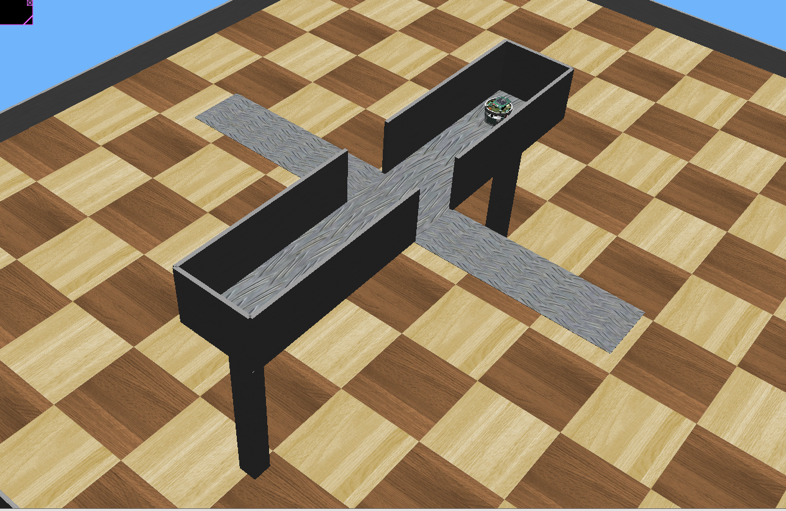
\includegraphics[width=.85\linewidth]{arena}
		\captionof{figure}{Simulation arena}
		\label{fig:arena}
	\end{minipage}%
\end{figure}

\subsection{Neural Network}

An Artificial Neural Network (ANN) is a system that is modelled on the biological brain, particularly on the hypothesis that mental activity consists primarily of electrochemical activity in networks of brain cells called neurons.

The signal output of a neuron can either cause excitation or inhibition in the neuron it is connected to. When a neuron sends an excitatory signal to another neuron, this signal is added to all of the other inputs of that neuron. If it exceeds a given threshold then it will cause the target neuron to fire an action potential, if it is below the threshold then no action potential occurs. \cite{Russell2009}

An ANN is comprised of nodes (neurons) connected by directed links. Each neuron receives input values either from the environment or from other neurons. Based on these inputs, the neuron calculates an output value by way of an activation function. Each link also has a numeric weight, known as a synaptic weight, associated with it, which determines the strength and sign of the connection. In effect, it is a distributed and parallel processor.

The network acquires knowledge from its environment through a learning process; a learning algorithm. The objective is to modify the network’s synaptic weights for the network to perform its desired function. The ability for synapses to modify is known as synaptic plasticity. \cite{Haykin2008}

Shown in Fig. \ref{fig:NN} is the utilised network.


\subsection{Genetic Algorithm}

A genetic algorithm is an iterative optimisation method based on natural selection that attempts to emulate the process of biological evolution. \cite{Fraser1970}

The algorithm begins by first creating a random set of possible solutions to the problem.

Each solution is called an \textit{individual} with its properties being termed \textit{chromosomes}. These chromosomes contain \textit{genes} and the complete set of possible solutions is the \textit{population}. 

Each individual in the population is evaluated based on how well it performs as a solution to the problem according to a fitness function. 

The result of this fitness function is a performance metric for the individual, and a selection operator utilises this metric to select individuals to create the next generation, a method termed \textit{reproduction}.

This is achieved through a genetic operator called a crossover, which is the mixing of a certain number of traits (genes) from each parent to produce an offspring. After this, random mutation of individuals in the population may occur. The algorithm terminates when a certain number of generations has been produced or when a solution with an acceptable level of fitness has been found. 



\section{Implementation}

\subsection{Arena setup}

In the model implemented, an ANN with fixed architecture was used, see Fig. \ref{fig:NN}. A genetic algorithm was used to optimise the weights of the ANN, evolving the desired rat behaviour. 

The simulated elevated plus maze was discretised into 15 positions as shown in Fig. \ref{fig:arena-disc}. This was inspired by a similar, proven solution detailed within \citeauthor{Costa201444} and \citeauthor{Costa2016102}. \cite{Costa201444} \cite{Costa2016102} GPS ranges from the E-puck were assigned EPM positions in order to provide the robot's position to the supervisor.


\begin{figure}[H]
	\centering
	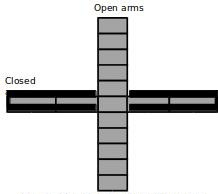
\includegraphics[width=0.7\linewidth]{arena-disc}
	\caption{Arena boundaries}
	\label{fig:arena-disc}
\end{figure}

\subsection{Robot controller}

The e-puck is controlled by a multilayer perceptron (MLP), shown in Fig. \ref{fig:NN} with arrows representing weighted links. 

The network's inputs are data from the circumferential IR proximity sensors. The outputs of the network specify wheel speed values. 

In terms of activation functions, every neuron uses a hyperbolic tangent function. This suited this application as this function’s output is between -1 and 1, which is ideal because wheel speeds can be negative. The output values are scaled by 1000, to match the possible range of values in wheel speeds.

Each layer of synaptic weights is represented by an N-by-N matrix, where each row is a neuron's connection's weights to the next layer. \cite{Seiffert2001} These individual sets of weights are encoded into another data structure, which contain the weights of each layer. 

\subsection{Evolution}

The network's weights are optimised by a genetic algorithm. 

Each individual of the population is evaluated by the GA. As stated, each individual is a separate robot controller (ANN), with different parameters (weights).

The population is initialised via a function that fills a matrix with uniformly distributed random numbers in the range of -1 to 1, which are the initial weights. The size of the initial population is dictated by the variable \emph{popsize}. 

The fitness of each individual is evaluated with a fitness function. At each time step, this takes in as input the position of the robot and the proximity sensor values. The fitness value assigned to a controller under evaluation is increased or decreased depending on whether it exhibited desirable or undesirable behaviour. The algorithm awards ``rat-like'' behaviour such as predominantly staying within the confines of the enclosure (anxious exploratory behaviour) and close to walls, and punishes falling off the arena, exploring the outer boundaries of the arm and wall collisions.

Each individual is evaluated after navigating through the virtual EPM for 30 seconds.

Successive generations are created through selection and reproduction of the previous generation.

Based on the fitness of these individuals, the best individuals are selected by elitism and the remaining individuals are selected through tournament selection. 

In elitism, a proportion of the best individuals are copied directly to the new generation, and the percentage for which this is done is dictated by the variable \textit{elitism}. 

In tournament selection, a number of individuals are chosen randomly, according to the variable \textit{tournamentSize}. These individuals are sorted by their fitness and the best two are chosen as parents. 

A new individual is reproduced using uniform crossover. In uniform crossover, there is a 50\% probability that the current gene is selected from one parent and not the other. 

Gaussian mutation is also applied with a probability dictated by the variable \textit{muteRate} (i.e. the number of individuals in a generation to be mutated) and with severity dictated by the variable \textit{severity} (i.e. the number of genes in the individual to be mutated). The variables mentioned above are all user definable.

When the best controller is evolved, the final generation of individuals is sorted by fitness and saved to an .xml file for analysis and reuse.

\subsection{Simulation supervisor}

The supervisor acts as a tool to guide and control the simulation. The user first sets the desired mode of operation (demo or evolution). Then the supervisor sets the time step of the current simulation as well as the duration of time each controller should run for, and resets the robot to its initial position.  



\section{Results} % The \section*{} command stops section numbering

A controller which mimicked the approach-avoidance behaviour of a rat in the EPM was successfully evolved.

With this controller, the virtual rat moves along the enclosed walls as it explores the maze, peeks onto the unenclosed positions but slowly turns away back into the enclosed space.

Shown in  Table \ref{tab:param} are the algorithm parameters used during evolution.

\begin{table}[H]
	\centering
	\begin{tabular}{llr}
		\toprule
		\multicolumn{2}{c}{Variables} \\
		\cmidrule(r){1-2}
		popsize & 50\\
		generations & 50\\
		tournamentSize & 3 \\
		elitism & 0.2\\
		muteRate & 0.02\\
		severity & 0.4\\
		\bottomrule
	\end{tabular}
	\caption{Genetic Algorithm Parameters}
	\label{tab:param} 	
\end{table}




\section{Discussion} % The \section*{} command stops section numbering

One of the first challenges faced was how to keep track of the position of the robot. Since the robot's position is required to evaluate the fitness of the controller, this was important. 

Due to its accuracy and ease of implementation, a GPS unit was decided upon. However an alternative would be to change the colour of the maze floor and use the ground sensors to detect the change in colour. In this way, the maze could still be discretised into zones. 

Using the method implemented, however, dividing the map into more positions could evolve a better controller.

Possibly, this method would be cheaper to implement in a real robot, since indoor GPS equipment is expensive. In addition, the ground sensors could be used to detect the absence of a floor at the edge of the unenclosed spaces, which would be analogous to a rat's whiskers. 

The neural network topology if fixed, however different architectures were considered.

A recurrent network was contemplated; however, this would have increased the complexity of both neural network computation and behavioural evolution. In addition to this, the running speed could be effected. However, more hidden layers and recurrence would represent more memory and information processing capability and would possibly result in evolving a good solution quicker. In addition to this, simultaneously evolving the weights, the architecture of the ANN, and the activation function would yield better results, at the cost of time and complexity.
 
Having fewer input nodes in the ANN and using less IR sensors on the robot was also considered, as rats use mostly the whiskers and eyes to gauge their environment.

Different numbers of outputs were considered too, such as four outputs, each representing a particular action for the robot to take, such as forward, left, right and stay in the same place. The final behaviour may have been more robotic than the one in our case, but the controller may have evolved quicker. 

Initially, the ANN was running on the robot, and the GA was running separately, through the supervisor. A two-way communication network was implemented wihtin the simulation, with the supervisor transmitting the weights to be tested to the robot and the robot transmitting its GPS co-ordinates to the supervisor. Unfortunately, this resulted in an extremely slow running speed, even using the simulation's ``fast mode''. Therefore, it was decided that the GA should run on the robot too. This increased the simulation speed ten fold. It wasthought this was probably due to the removal of the emitter and receiver previously needed when transmitting data between the robot and the supervisor.
 
For the fitness function, an extra component was implemented, which recorded the number of times the e-puck visited each position, and punished the individual if it visited one position frequently and never visited others. However, this seemed to have no effect on the evolution of the controller, and it was decided that assigning more points to positions further away from the starting position was simpler and more effective.

For more robust evolution, the robot's initial starting position could also be altered.



\section{Conclusion} % The \section*{} command stops section numbering

This experiment aimed to examine an application of evolutionary robotics techniques. A computational model of a rat exhibiting the aproach/avoidance conflict was obtained. In particular, a genetic algorithm was used to evolve the controller of an E-puck robot within simulation.

The behaviour exhibited by the robot is similar to that of a real rat, though some areas where improvement could be were highlighted.

Further work could be done within the genetic algorithm by modifying the type of selection and crossover used to generate a new population, as well as changing the population and generation size and allowing evolution to progress for longer. In addition, the hardware used by the robot to operate could be evolved. This could be achieved by giving the algorithm access to all available sensors and letting the evolution process select which sensors are best suited. This coud lead to efficiency increases.


%----------------------------------------------------------------------------------------
%	REFERENCE LIST
%----------------------------------------------------------------------------------------
\phantomsection
\bibliographystyle{unsrt}
\bibliography{sample}

%----------------------------------------------------------------------------------------

\end{document}